\section{Adding an Environment}
\label{sec:adding_env}
So far we have implicitly assumed a fully connected network amongst agents, where each agent can see and knows every other agent. This is a valid environment in accordance with the System Dynamics inspired implementation of the SIR model, but it does not show the real advantage of ABS to situate agents within arbitrary environments. Often, agents are situated within a discrete 2D environment which is simply a finite $N*M$ grid with either a Moore or von Neumann neighbourhood (Figure \ref{fig:abs_neighbourhoods}). Agents are either static or can move freely around with cells allowing either single or multiple occupants.

We can directly map the SIR model to a discrete 2D environment by placing the agents on a corresponding 2D grid with an unrestricted neighbourhood. The behaviour of the agents is the same but they select their interactions directly from the read-only environment, which will be passed to the agents as input. This allows agents to read the states of all their neighbours, which tells them if a neighbour is infected or not. To show the benefit over the System Dynamics approach  and for purposes of a more interesting approach, we restrict the agents to a Moore neighbourhood (Figure \ref{fig:moore_neighbourhood}).

\begin{figure}
\begin{center}
	\begin{tabular}{c c}
		\begin{subfigure}[b]{0.3\textwidth}
			\centering
			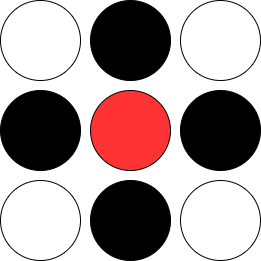
\includegraphics[width=0.5\textwidth, angle=0]{./fig/timedriven/neumann.png}
			\caption{von Neumann}
			\label{fig:neumann_neighbourhood}
		\end{subfigure}
    	&
		\begin{subfigure}[b]{0.3\textwidth}
			\centering
			
\includegraphics[width=0.5\textwidth, angle=0]{./fig/timedriven/moore.png}
			\caption{Moore}
			\label{fig:moore_neighbourhood}
		\end{subfigure}
    \end{tabular}
	\caption[Common neighbourhoods in discrete 2D environments of ABS]{Common neighbourhoods in discrete 2D environments of ABS.}
	\label{fig:abs_neighbourhoods}
\end{center}
\end{figure}

We also implemented this spatial approach in Java using the well-known ABS library RePast \cite{north_complex_2013}, to compare with a state of the art approach, and came to the same results as shown in Figure \ref{fig:sir_dunai}. This supports the hypothesis that our pure functional approach can produce such results as well and compares positively to the state of the art in the ABS field.

\subsection{Implementation}
\label{sub:timedriven_thirdstep_impl}
We start by defining the discrete 2D environment, for which we use an indexed two dimensional array \cite{array_hackage}. Each cell stores the agent state of the last time step. Consequently we use the \texttt{SIRState} as type for the array data. Additionally, we redefine the agent signal function to take the structured environment \texttt{SIREnv} for the input instead of the list of all agents as in the previous step. For the output we keep the \texttt{SIRState}, which is the state the agent is in currently. Moreover, we run in the \texttt{Rand} Monad as introduced before to avoid the random-number correlation. 

\begin{HaskellCode}
type Disc2dCoord = (Int, Int)
type SIREnv      = Array Disc2dCoord SIRState
type SIRAgent g  = SF (Rand g) SIREnv SIRState
\end{HaskellCode}

The environment is not returned as the output because the agents do not directly manipulate the environment, they only read from it. Again, this enforces the semantics of the \textit{parallel} update strategy, through the types where the agents can only see the previous state of the environment as well as the actions of other agents reflected in the environment only in the next step.

We could have chosen to use a \texttt{StateT} transformer with the \texttt{SIREnv} as state, instead of passing it as input. The agents would have then been able to arbitrarily read and write, but this would have violated the semantics of our model because the actions of agents would have become visible within the same time step.

The implementation of the susceptible, infected and recovered agents is almost the same with only the neighbour querying now in a slightly different way. 

Stepping the simulation needs a new approach, because in each step we need to collect the agent outputs and update the environment for the next step. For this we implemented a separate \texttt{MSF}, which receives the coordinates for every agent to be able to update the state in the environment after the agent was run. It is important to understand that we need to use \texttt{mapM} to run the agents because we are now running in the context of the \texttt{Rand} Monad. This has the consequence that the agents are, in fact, run sequentially one after the other. But, because they cannot see the other agents actions nor observe changes in the read-only environment, it is \textit{conceptually} a \textit{parallel} update strategy where agents run in lock-step, isolated from each other at conceptually the same time.
  
\begin{HaskellCode}
simulationStep :: RandomGen g => [(SIRAgent g, Disc2dCoord)] -> SIREnv
               -> SF (Rand g) () SIREnv
simulationStep sfsCoords env = MSF (\_ -> do
  let (sfs, coords) = unzip sfsCoords 
  -- run agents sequentially but with read-only environment
  ret <- mapM (`unMSF` env) sfs
  -- construct new environment from all agent outputs for next step
  let (as, sfs') = unzip ret
      env' = foldr (\ (a, coord) envAcc -> updateCell coord a envAcc) 
                   env (zip as coords)

      sfsCoords' = zip sfs' coords
      cont       = simulationStep sfsCoords' env'
  return (env', cont))
 
updateCell :: Disc2dCoord -> SIRState -> SIREnv -> SIREnv
\end{HaskellCode}

\subsection{Results}
We implemented rendering of the environments using the  \href{http://hackage.haskell.org/package/gloss}{gloss}~\cite{gloss_library} library which enabled us to cycle arbitrarily through the steps and inspect the spreading of the disease over time visually as seen in Figure \ref{fig:sir_dunai}.

\begin{figure}
\begin{center}
	\begin{tabular}{c c}
		\begin{subfigure}[b]{0.4\textwidth}
			\centering
			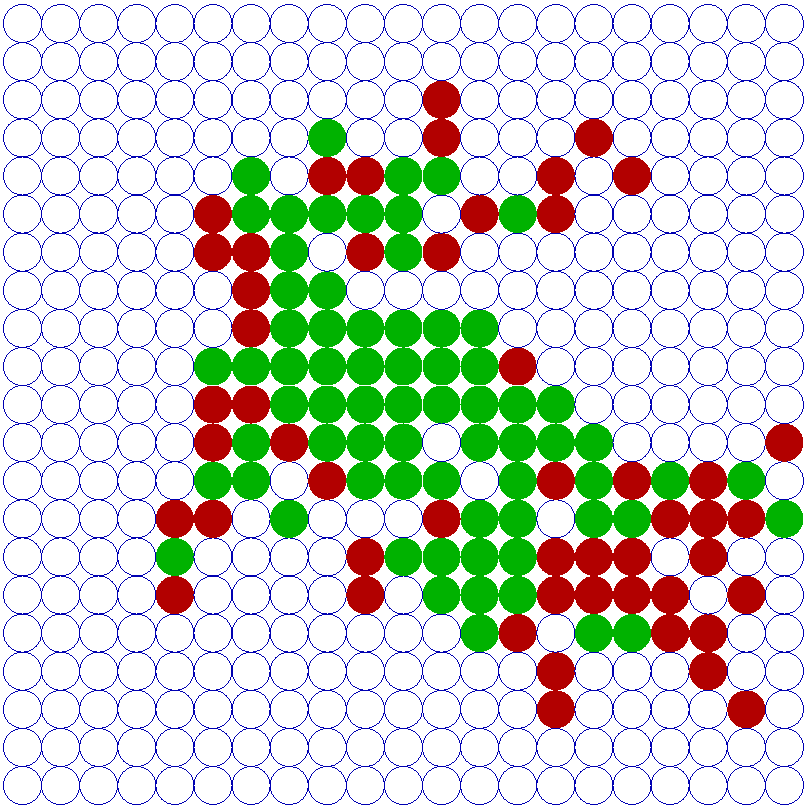
\includegraphics[width=1\textwidth, angle=0]{./fig/timedriven/SIR_Dunai/SIR_Dunai_dt001_environment.png}
			\caption{Environment at $t = 50$}
			\label{fig:sir_dunai_env}
		\end{subfigure}
    	
    	&
  
		\begin{subfigure}[b]{0.43\textwidth}
			\centering
			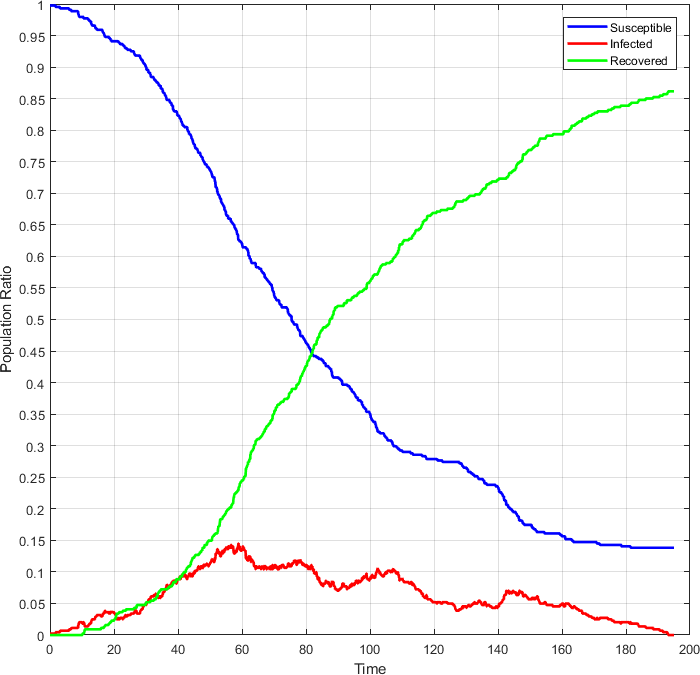
\includegraphics[width=1\textwidth, angle=0]{./fig/timedriven/SIR_Dunai/SIR_Dunai_dt001.png}
			\caption{Dynamics over time}
			\label{fig:sir_dunai_env_dynamics}
		\end{subfigure}
	\end{tabular}
	
	\caption[Simulating the agent-based SIR model on a 21x21 2D grid with Moore neighbourhood]{Simulating the agent-based SIR model on a 21x21 2D grid with Moore neighbourhood (Figure \ref{fig:moore_neighbourhood}), a single infected agent at the center and same SIR parameters as in Figure \ref{fig:sir_sd_dynamics}. Simulation run until $t = 200$ with fixed $\Delta t = 0.01$. Last infected agent recovers around $t = 194$. The susceptible agents are rendered as blue hollow circles for better contrast.}
	\label{fig:sir_dunai}
\end{center}
\end{figure}

The dynamics of the spatial SIR simulation, which are seen in Figure \ref{fig:sir_dunai_env_dynamics}, look quite different from the reference dynamics of Figure \ref{fig:sir_sd_dynamics}. This is due to a much more restricted neighbourhood, resulting in far fewer infected agents at a time, as well as a lower number of recovered agents at the end of the epidemic. This result then indicates that fewer agents got infected overall.

\subsection{Discussion}
Introducing a structured environment with a Moore neighbourhood shows the ability of ABS to place the heterogeneous agents in a generic environment. This scenario shows the fundamental advantage of an agent-based approach over other simulation methodologies and allows us to simulate much more realistic scenarios.

An environment is not restricted to a discrete 2D grid and can be anything from a continuous N-dimensional space to a complex network. One only needs to change the type of the environment and agent input and provide corresponding neighbourhood querying functions in order to make change of this kind. 